% ============================================================================
% EKLER
% ============================================================================
% 2026-10-31 (konsey turu, T3): yeni dosya; EN sections/07_appendix.tex aynasi.
% Govdeden tasinanlar (EN ile ayni):
%   Ek A app:behavior   - eski 04 G (uc okuma), epsilon taramasi, eski TGR
%                         sonucu; tanimlar eski 03'ten kisaltilarak.
%   Ek B app:selection  - eski 04 F (secim kurali) ve H (varyans kaynaklari);
%                         subsec:selection etiketi burada korunur.
%   Ek C app:registrations - eski CIFAR-100 ve L2 kayitli ongoruleri.
% Dusenler: fig:gradient_analysis, fig:gradient_heatmap, fig:attention_layers,
% tab:tgr, tab:cifar100_results, tab:l2_results.
% tab:feature_degradation'in "Tum jetonlar" sutunu EN ile birlikte dustu
% (foy Tablo 10'da duruyor; metin yalniz CLS ve yama ortalamasini kullanir).
% Sekiller final_tr surumleri (ayni betik, --lang tr, EN final ile ayni uretim).
% Her sayi results/C1_REFERANS_FOYU.md'den; paragraf ustunde "% FOY:" yorumu.
\appendices

\section{Çiftin Davranışsal Ölçümleri}
\label{app:behavior}

% FOY:Epsilon taramasi:356,357,358,359,360,361,362,364 (tarama), 366-370 (Tablo I ile fark)
CNN'in ViT üzerindeki üstünlüğü küçük bütçelerde en geniştir ($2/255$ için $\%64{,}10$'a karşı $\%77{,}30$) ve $16/255$'te daralır ($\%12{,}16$'ya karşı $\%20{,}38$; Şekil~\ref{fig:epsilon_sweep}).

% FOY:Epsilon taramasi:371,373 (Tablo I ile fark, 8/255)
\begin{figure}[!t]
\centering
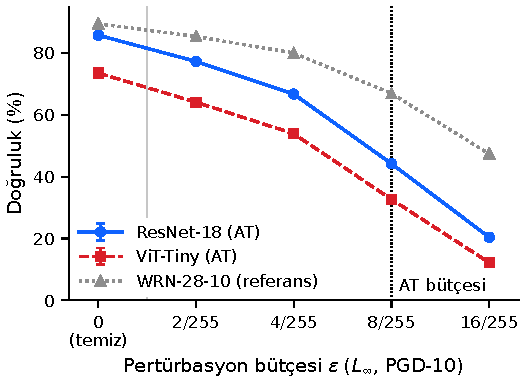
\includegraphics[width=\columnwidth]{../figures/final_tr/fig2_epsilon_sweep.pdf}
\caption{CIFAR-10 test kümesinde PGD-10 gürbüz doğruluğunun bütçe $\eps$'a göre değişimi; üç koşunun ortalaması verilmiş olup hata çubukları işaretçilerden dardır ve $\eps=0$ temiz doğruluğu göstermektedir. Bu ayrı değerlendirme $8/255$ bütçesinde Tablo~\ref{tab:main_results} değerlerinden en çok $0{,}08$ puan ayrılmaktadır.}
\label{fig:epsilon_sweep}
\end{figure}

% KAYNAK: eski 03_methodology.tex (Gradient Analysis, Spatial Locality Metrics; tanimlar)
% FOY:Gradyan yapisi:90,91,92,93,95,97,99,100,101,102 ; Tablo 8 ek sutunlari:254,262 ; M8.10:1321 (kosum basina 500 goruntu)
% FOY:M8.10:1325,1326,1327,1328,1330 ; Tablo 9 ek sutunlari:279,280,281,282
Örnek başına kayıpların girdi gradyanları her koşuda $500$ test görüntüsü üzerinde ölçülmüştür. Seyreklik, ölçekten bağımsız üç ölçüyle, yani Hoyer seyrekliği, Gini katsayısı ve örnek başına en büyük değerin \%1'inin altında kalan bileşenlerin kesriyle~\cite{hurley2009comparing}, mekânsal lokalite ise normalleştirilmiş kanal toplamı enerji haritası üzerinde puanlanmıştır (Tablo~\ref{tab:spatial}). CNN gradyanları her koşuda üç ölçünün üçünde de daha seyrektir (Tablo~\ref{tab:gradient}). Koşu içindeki eşleştirilmiş testler sıfır hipotezini reddetmiştir (Holm $p \leq 2{,}2\times10^{-12}$). Ancak mimari bir iddianın gerektirdiği birim olan koşu düzeyinde Holm düzeltmesinden sonra $p = 0{,}108$ kalmaktadır. Bu nedenle sıralama yeniden üretilebilir olmakla birlikte anlamlı değildir. Söz konusu sıralamayı çekişmeli eğitim üretmektedir. Temiz eğitildiğinde daha seyrek model ViT'tir (Hoyer $0{,}347$ değerine karşı $0{,}380$) ve CIFAR'a özgü bir ViT, büyütülen ViT'ten daha az seyrektir. Mutlak hizalanma ViT'te daha yüksektir (koşu düzeyinde $p = 0{,}0009$), işaretli hizalanma ise iki modelde de $0{,}0014$ ya da altında kalmaktadır. Mekânsal betimleyicilerin hiçbiri koşu düzeyinde farklılaşmamış (Holm $p$ değerleri $0{,}40$ ile $0{,}54$ arasında) ve bunların ikisi koşular arasında işaret değiştirmiştir. Dolayısıyla CNN'in daha seyrek gradyanları daha lokalize değildir.

% FOY:Gradyan yapisi:90,91,92,93 ; Tablo 8 ek sutunlari:254,255,262,263,264,265 ; M8.10:1321 (n = 500)
\begin{table}[!t]
\centering
\caption{Gradyan karakteristikleri (koşu başına $n=500$ görüntü; üç koşu üzerinden ortalama$\pm$SS). Yerel kontrol, sabit bölme protokolünden önceye ait ve CIFAR'a özgü tek bir ViT kontrol noktasıdır ($4\times4$ yama).}
\label{tab:gradient}
\footnotesize
\setlength{\tabcolsep}{2.5pt}
\begin{tabular}{lccc}
\toprule
\textbf{Metrik} & \textbf{ResNet-18 AT} & \textbf{ViT-Tiny AT} & \textbf{ViT (yerel)} \\
\midrule
Hoyer seyrekliği & 0,4928$\pm$0,0120 & 0,4561$\pm$0,0055 & 0,4046 \\
Gini katsayısı & 0,6498$\pm$0,0089 & 0,6099$\pm$0,0051 & 0,5712 \\
Maks.\ \%1 altı kesir & 0,3477$\pm$0,0210 & 0,2682$\pm$0,0090 & 0,1785 \\
Hizalanma (mutlak) & 0,0378$\pm$0,0009 & 0,0562$\pm$0,0004 & 0,0794 \\
Hizalanma (işaretli) & 0,0010$\pm$0,0003 & 0,0004$\pm$0,0001 & -- \\
\bottomrule
\end{tabular}
\end{table}

% FOY:C5:125,131,132,133,134 ; Tablo 9 ek sutunlari:279,280,281,282 (fark SD, Holm p)
\begin{table}[!t]
\centering
\caption{Girdi gradyanlarının mekânsal lokalitesi (koşu başına $n=500$; üç koşu üzerinden ortalama$\pm$SS). $p$, koşu başına üç eşleştirilmiş fark üzerinde yapılan tek örneklem $t$ testidir ve dört ölçü üzerinden Holm düzeltmesi uygulanmıştır.}
\label{tab:spatial}
\scriptsize
\setlength{\tabcolsep}{1.6pt}
\begin{tabular}{lcccc}
\toprule
\textbf{Ölçüt} & \textbf{ResNet-18} & \textbf{ViT-Tiny} & \textbf{Fark (R$-$V)} & \textbf{$p$ (Holm)} \\
\midrule
\%50 enerji alanı & 0,0378$\pm$0,0017 & 0,0397$\pm$0,0010 & $-$0,0019$\pm$0,0027 & 0,54 \\
\%90 enerji alanı & 0,2345$\pm$0,0078 & 0,2570$\pm$0,0067 & $-$0,0224$\pm$0,0133 & 0,40 \\
Mekânsal entropi (nat) & 5,2014$\pm$0,0387 & 5,2524$\pm$0,0197 & $-$0,0509$\pm$0,0580 & 0,54 \\
Moran $I$ & 0,4141$\pm$0,0132 & 0,3941$\pm$0,0024 & $+$0,0200$\pm$0,0156 & 0,47 \\
\bottomrule
\end{tabular}
\end{table}

% KAYNAK: eski 03_methodology.tex (Token Aggregation, Attention Metrics, Feature Degradation Metrics)
% FOY:C4:110,111,113,120,122,123 ; Tablo 10:288-323 ; Dikkat entropisi:348,350
% FOY:Dikkat entropisi TOST:1113,1138,1139
Öznitelik kayması, modelin kendi PGD-10 saldırısı altında her artık blok çıkışında temizden çekişmeliye kosinüs benzerliği olarak ölçülmüştür (koşu başına $n = 1.000$). ViT'te kayma kademelidir ve öznitelik normlarını \%0,45 içinde bırakırken CNN'de son aşamanın ilk bloğunda yoğunlaşmakta ve $-\%13{,}14\pm1{,}89$ norm değişimiyle birlikte gelmektedir (Tablo~\ref{tab:feature_degradation}). Minimumlarında, yani 11. ve 9. bloklarda, CLS jetonu yama jetonu ortalamasının yaklaşık üç katı kaymaktadır. Başlar üzerinden ortalanmış CLS dikkatinin entropisi ise değişmemektedir. Katman başına en büyük değişim, temiz değerler $4{,}61$ ile $5{,}11$ nat arasındayken $0{,}0045$ nat olarak ölçülmüş ve $\pm0{,}05$ nat marjla koşu düzeyinde yapılan TOST, $12$ katmanın tamamında eşdeğerliği kabul etmiştir (Şekil~\ref{fig:feature_degradation}). Dikkat haritasının yer değiştirmesi derinlikle $0{,}028$ düzeyinden $0{,}084$ düzeyine büyümüştür. Dolayısıyla saldırı dikkati genişletmeden yeniden yönlendirmektedir. Son blok kayması yanıltılan ve yanıltılmayan görüntüleri ayırmamaktadır (koşu düzeyinde ViT için $p = 0{,}20$, CNN için $0{,}080$).

% FOY:Tablo 10:288-299,300-303 (ViT), 317-324 (ResNet)
\begin{table}[!t]
\centering
\caption{Her modelin kendi PGD-10 saldırısı altında artık blok çıkışlarında temizden çekişmeliye kosinüs benzerliği (koşu başına $n=1.000$; üç koşunun ortalaması).}
\label{tab:feature_degradation}
\footnotesize
\setlength{\tabcolsep}{3pt}
\begin{tabular}{lcc@{\hspace{10pt}}lc}
\toprule
\multicolumn{3}{c}{\textbf{ViT-Tiny AT}} & \multicolumn{2}{c}{\textbf{ResNet-18 AT}} \\
\cmidrule(lr){1-3} \cmidrule(lr){4-5}
\textbf{Blok} & \textbf{CLS} & \textbf{Yama ort.} & \textbf{Aşama.blok} & \textbf{Kosinüs} \\
\midrule
1 & 0,9993 & 0,9980 & 1.1 & 0,9951 \\
2 & 0,9950 & 0,9959 & 1.2 & 0,9918 \\
3 & 0,9902 & 0,9940 & 2.1 & 0,9879 \\
4 & 0,9873 & 0,9919 & 2.2 & 0,9853 \\
5 & 0,9845 & 0,9904 & 3.1 & 0,9753 \\
6 & 0,9814 & 0,9894 & 3.2 & 0,9607 \\
7 & 0,9782 & 0,9885 & 4.1 & 0,8777 \\
8 & 0,9743 & 0,9875 & 4.2 & 0,9108 \\
9 & 0,9703 & 0,9870 & & \\
10 & 0,9661 & 0,9872 & & \\
11 & 0,9604 & 0,9874 & & \\
12 & 0,9663 & 0,9915 & & \\
\bottomrule
\end{tabular}
\end{table}

% FOY:Dikkat entropisi TOST:1113 ; Dikkat entropisi:334-345,350
\begin{figure}[!t]
\centering
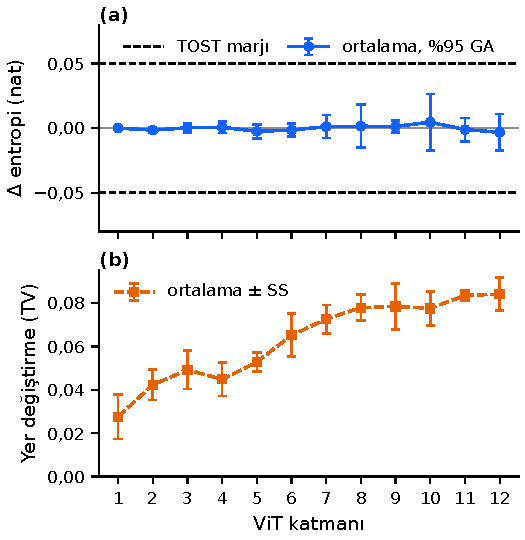
\includegraphics[width=\columnwidth]{../figures/final_tr/fig5b_attention_entropy.pdf}
\caption{(a) Saldırı altında ViT CLS dikkat entropisindeki katman başına değişim; üç koşunun ortalaması ve \%95 $t$ aralıkları kesikli çizgiyle gösterilen $\pm0{,}05$ nat eşdeğerlik marjının içinde kalmaktadır. (b) CLS dikkat haritasının katman başına toplam varyasyon yer değiştirmesi (koşular üzerinden ortalama$\pm$SS).}
\label{fig:feature_degradation}
\end{figure}

% FOY:C2:143,144,146 ; M8.4:1196 (ayri MI-FGSM kosusu, ViT->CNN 15.42)
% KAYNAK: eps 8/255, 10 adim (tasarim sabiti)
Çift üzerinde daha önce yapılan eşlenmiş bütçeli bir karşılaştırma Bölüm~\ref{subsec:attack_side} ile uyumludur. Jeton gradyanı düzenlileştirme~\cite{zhang2023tgr}, ViT kaynağından MI-FGSM~\cite{dong2018boosting} saldırısına göre daha kötü transfer olmuştur (hedef doğru protokolünde $\%15{,}71\pm0{,}60$ değerine karşı $\%12{,}70\pm0{,}41$). Bu karşılaştırma, Bölüm~\ref{subsec:transfer} içindeki MI-FGSM denetiminden ($\%15{,}42\pm0{,}52$) ayrı bir koşuda yapılmıştır.

\section{Kontrol Noktası Seçimi ve Varyans Kaynakları}
\label{app:selection}
\label{subsec:selection}

% FOY:M8.7:1269,1273,1274,1286,1287,1293
Sabit bir yörüngeden son kontrol noktasının yalnız nasıl seçildiği değiştirildiğinde (doğrulama bölmesi, sabır ve eğri yumuşatma; on sekiz bileşim) PGD-10 doğruluğu tohum başına ResNet'te $2{,}62$ ile $2{,}85$, ViT'te $1{,}58$ ile $2{,}09$ puan oynamıştır. Bu yayılım puan olarak verilmiş ve bilinçli olarak tohum düzeyi yayılıma oran biçiminde verilmemiştir. Bu tercihin nedeni, söz konusu oranın referans hücreye bağlı olarak ResNet'te $0{,}67$ ile $3{,}38$, ViT'te $0{,}63$ ile $7{,}38$ arasında değişmesidir. Seçim yolları kararsızken sonuçlar kararlı kalabilmektedir. CIFAR-100'de seçilen epok ResNet tohumları arasında $25$ epok değişmiş, buna karşın test PGD-10 standart sapması $0{,}32$ puanda kalmıştır.

% FOY:Secim kuralinin asimetriye etkisi:799,808,813,814,815,816,817,818,825 ; M8.14:1390,1392
Seçilenlerden yirmi epok sonraki son kontrol noktalarında üç eğitim çiftinin temiz farkı $12{,}26\pm0{,}90$ yerine $10{,}55\pm0{,}59$ puan, dört protokollü yayılımı ise $12{,}84\pm0{,}34$ puan olarak ölçülmüştür. CNN$\rightarrow$ViT işareti her protokolde korunmuş ve özdeşlik öncülü bozulmamıştır ($p \geq 0{,}9915$).

% FOY:TabloI:16,17 ; TabloIII:159,160,161,162,163 ; M8.8:1295-1309
% FOY:M10.7:2049,2050 (saldiri tohumu SD'si; ilk C1 cifti 1001/2001, ilk 1000 goruntu, 3 saldiri tohumu,
% artefakt alani np.std ddof 0: CNN 0.05, ViT 0.00 puan). 2026-10-31: TODO(foy) kapandi.
Karşılaştırmaları dört varyans kaynağı etkilemektedir. Bir tohum çiftinin ilk $1.000$ test görüntüsünde üç saldırı tohumu üzerinden hesaplanan gürbüz doğruluk standart sapması CNN'de $0{,}05$, ViT'te $0{,}00$ puandır. Eğitim koşuları doğruluğu en çok $0{,}55$ puanlık bir standart sapmayla, transfer asimetrisini ise protokole bağlı olarak $0{,}23$ ile $1{,}27$ puan arasında oynatmaktadır. Sabit bir tohum çiftinde protokol asimetriyi $15{,}01\pm0{,}84$ puan, seçim kuralı ise yayılımı yaklaşık iki puan oynatmaktadır (Bölüm~\ref{subsec:transfer}). İki serbestlik derecesiyle $\chi^2$ aralığı çok geniş kaldığından protokol yayılımının koşu yayılımına oranı kanıt olarak kullanılmamıştır.

\section{CIFAR-100 ve \texorpdfstring{$L_2$}{L2} Bütçesi için Kayıtlı Öngörüler}
\label{app:registrations}

% FOY:TabloIII:159-163 (CIFAR-100 sutunu) ; Basarili-kaynak siki ve gevsek:240 (10.45) ; M8.2:1171
% FOY:M10.7:2058,2060,2062 (CIFAR-100 C3 hedef temiz hatalari 36.15 ve 36.36; en kucuk ara 0.21). 2026-10-31: TODO(foy) kapandi.
Herhangi bir CIFAR-100 ölçümünden önce üç yönlü öngörü ve üç uç nokta bandı kayda alınmıştır. Öngörülen işaret on iki ölçümün tamamında tutmuştur. CIFAR-10'dakinden daha büyük bir yayılım öngörüsü, o sırada $10{,}45$ puan olarak verilen CIFAR-10 yayılımını referans almıştır. Ölçülen $13{,}83$ bu sayıyı aşmakta, ancak katı başarılı kaynak okumasındaki yayılımı ($15{,}01$) aşmadığı için öngörü başarısız sayılmıştır. Üçüncü öngörü, koşulsuz oranların koşullu oranlardan sapmasının hedefin temiz hatasıyla büyüyeceğini ileri sürmüş ve pozitif bir eğim vermiştir ($+0{,}656$, $r_{\mathrm{P}} = 0{,}931$). Ne var ki üç hedeften ikisinin temiz hataları neredeyse eşittir ($\%36{,}15$ ve $\%36{,}36$) ve bu öngörü bu tasarımda sınanamaz.

% FOY:Turetilmis:229 (43.17 +- 1.10) ; M8.5:1235,1236,1245,1246,1247 ; M8.7:1280
% KAYNAK: results/q1_research/E1_PILOT_KAPISI.md (on kayitli ViT temiz bandi 33-40)
ViT için öngörülen temiz doğruluk bandı ($\%33$ ile $\%40$), ölçülen $\%43{,}17\pm1{,}10$ değeriyle tutturulamamıştır. Bunun nedeni, ViT'in çekişmeli eğitim altında temiz ön eğitim doğruluğunun $0{,}885$'ini korurken ResNet'in $0{,}802$'sini korumasıdır. İki çekişmeli uç nokta da bantlarının içine düşmüştür. Ancak bandın sınırına olan paylar $0{,}22$ puan (AutoAttack) ve $0{,}48$ puandır (PGD-10). Bu paylar, kontrol noktası seçiminin bu veri kümesinde PGD-10 doğruluğunda yol açtığı $0{,}18$ ile $1{,}83$ puanlık oynamanın altında kalmaktadır (Ek~\ref{subsec:selection}).

% FOY:TabloIII:159-164 (L2 sutunu) ; M8.2:1172,1173 ; M8.11:1337-1341 (McNemar, en buyuk p 2.729e-58)
% KAYNAK: L2 eps = 0.5 (tasarim sabiti)
Aynı CIFAR-10 kontrol noktalarında $\eps = 0{,}5$ büyüklüğünde bir $L_2$ bütçesi altında protokol yayılımı $10{,}92\pm0{,}82$ puana inmiş ve işaret on iki ölçümün tamamında pozitif kalmıştır. Böylece kayıtlı üç öngörüden ikisi tutmuştur. Üçüncüsü, Denklem~\eqref{eq:raw_identity} sağlandığı anda başarısız olamaz ve uydurulan $+0{,}914$ eğimi $1 - r_{\text{koş}}$ değerini kestirmektedir. On sekiz yön yalnız yedi farklı hedef hata değeri aldığı ve yönlerin altısı sabit WideResNet hedefini paylaştığı için korelasyon yerine eğim raporlanmıştır. CNN mutlak üstünlüğünü korumaktadır (tohum çifti başına McNemar $p \leq 2{,}729\times10^{-58}$).

\section{CIFAR-10 Ailelerinin Keşifsel Yeniden Çözümlemeleri}
\label{app:exploratory}

% Kaynak notu (FOY grubu degil): foy M12.1 satir 2218-2220 ve M12.3 satir 2302-2320 (etiket, tanim, mimari
% dogrulama); sapma kaydi results/q1_research/ONKAYIT_SAPMALAR.md satir 89 ve sonrasi. 2026-10-31 son gecis.
Buradaki iki çözümleme, sonuçlar ve bir iç değerlendirme görüldükten sonra belirlenmiştir. İkisi de dondurulmuş fonksiyonları değiştirmeden kullanmakta ve hiçbir karar ailesine girmemektedir. Tablo~\ref{tab:simple_effects}, $2\times2$ karşıtlıklarını basit etkilerine ayırmaktadır. Tablo~\ref{tab:reduced_panel} ise sekiz bloklu ResNet-18 dizilimine sahip dört panel üyesini dışarıda bırakmaktadır. Geriye kalan üç üye kayıtlı en az beş üye kuralının altında kaldığından dondurulmuş betik, isteğe bağlı üç üye bayrağıyla koşulmuştur.

% FOY:M12.1:2228-2239,2245-2256 (A2: birlesik varyansli t %90, Welch %90, logit; kesifsel, on kayit disi)
\begin{table}[!t]
\centering
\caption{CIFAR-10'da $2\times2$ tasarımın basit etkileri (bölünmüş yarı, log ölçeği; keşifsel). Mimari etkisi bir satır içinde ViT eksi ResNet, başlatma etkisi ise bir mimari içinde ImageNet eksi sıfırdan farkıdır; kayıtlı karşılıklar parantez içinde verilmiştir. Birleştirilmiş varyanslı aralıklar Tablo~\ref{tab:fb4} ile aynı biçimde hesaplanmış, Welch aralıkları yalnız karşıtlığa giren hücreleri kullanmıştır.}
\label{tab:simple_effects}
\scriptsize
\setlength{\tabcolsep}{2.5pt}
\begin{tabular}{lcccc}
\toprule
\textbf{Karşıtlık} & \textbf{Kestirim} & \textbf{Birl.\ \%90 GA} & \textbf{Welch \%90 GA} & \textbf{Logit} \\
\midrule
\multicolumn{5}{l}{\textit{Panel benzerliği $\sigma$}} \\
Mimari, sıfırdan (H1) & $-$0,364 & [$-$0,415; $-$0,314] & [$-$0,472; $-$0,256] & $-$0,498 \\
Mimari, ImageNet & $-$0,104 & [$-$0,159; $-$0,049] & [$-$0,318; $+$0,109] & $-$0,144 \\
Başlatma, ViT & $+$0,270 & [$+$0,219; $+$0,320] & [$+$0,043; $+$0,496] & $+$0,372 \\
Başlatma, ResNet & $+$0,009 & [$-$0,046; $+$0,065] & [$-$0,084; $+$0,102] & $+$0,018 \\
Etkileşim (H2) & $+$0,260 & [$+$0,186; $+$0,335] & [$+$0,113; $+$0,407] & $+$0,354 \\
Mimari ana etkisi & $-$0,234 & [$-$0,271; $-$0,197] & [$-$0,308; $-$0,161] & $-$0,321 \\
\midrule
\multicolumn{5}{l}{\textit{Yönlü terim $\rho$}} \\
Mimari, sıfırdan & $+$0,070 & [$+$0,039; $+$0,101] & [$-$0,031; $+$0,172] & $-$0,061 \\
Mimari, ImageNet & $-$0,064 & [$-$0,098; $-$0,030] & [$-$0,140; $+$0,013] & $-$0,112 \\
Başlatma, ViT (S2) & $-$0,130 & [$-$0,161; $-$0,099] & [$-$0,182; $-$0,078] & $-$0,034 \\
Başlatma, ResNet & $+$0,004 & [$-$0,030; $+$0,038] & [$-$0,122; $+$0,130] & $+$0,017 \\
Etkileşim & $-$0,134 & [$-$0,180; $-$0,088] & [$-$0,208; $-$0,060] & $-$0,051 \\
Mimari ana etkisi (H3) & $+$0,003 & [$-$0,020; $+$0,026] & [$-$0,034; $+$0,041] & $-$0,087 \\
\bottomrule
\end{tabular}
\end{table}

% FOY:M12.3:2335-2340,2344,2345,2351-2356,2362-2368 (A10: 3 ve 7 uyeli panel; kesifsel, on kayit disi)
\begin{table}[!t]
\centering
\caption{Dondurulmuş kurallar altında CIFAR-10 aileleri: kayıtlı panelle ve keşifsel olarak ResNet-18 türevleri çıkarılmış panelle (Engstrom2019 RN-50, Carmon2019 ve Gowal2020 WRN-28-10). Aralıklar Tablo~\ref{tab:panel_tests} ve~\ref{tab:fb4} ile aynı biçimde hesaplanmıştır. H2'nin logit kestirimi pozitif kalmaktadır ($+0{,}390$).}
\label{tab:reduced_panel}
\scriptsize
\setlength{\tabcolsep}{1.6pt}
\begin{tabular}{lccccc}
\toprule
& \multicolumn{2}{c}{\textbf{Yedi üye}} & \multicolumn{2}{c}{\textbf{Üç üye}} & \\
\cmidrule(lr){2-3} \cmidrule(lr){4-5}
\textbf{Sınama} & \textbf{Kestirim} & \textbf{\%90 GA} & \textbf{Kestirim} & \textbf{\%90 GA} & \textbf{Karar} \\
\midrule
H1 & $-$0,364 & [$-$0,415; $-$0,314] & $-$0,412 & [$-$0,465; $-$0,359] & destek \\
H2 & $+$0,260 & [$+$0,186; $+$0,335] & $+$0,295 & [$+$0,216; $+$0,373] & destek \\
H3 & $+$0,003 & [$-$0,020; $+$0,026] & $+$0,004 & [$-$0,021; $+$0,029] & eşdeğer \\
K-a & 0,936 & [0,925; 0,948] & 0,921 & [0,905; 0,936] & destek \\
K-b & $+$0,012 & [$-$0,007; $+$0,031] & $+$0,018 & [$-$0,008; $+$0,044] & eşdeğer \\
K-c & $+$0,566 & [$+$0,537; $+$0,604] & $+$0,673 & [$+$0,641; $+$0,714] & destek \\
Bölge & O1 & & O1 & & \\
\bottomrule
\end{tabular}
\end{table}
